\subsubsection{Graphische Beschreibung der Ionenstärkeabhängigkeit von k}

\begin{figure}[H]
	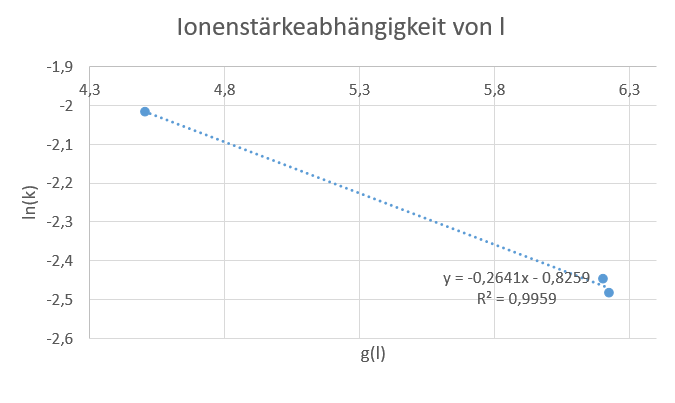
\includegraphics[width=\linewidth]{C:/Users/josefk/Desktop/kinetik/src/img/ionenstärkeabhängigkeitVonK.PNG}
\end{figure}


\begin{table}[H]
	\centering
    \begin{tabular}{lll}
        \toprule
        Lösung & ln(k)   & g(l)        \\
        \midrule
		2      & -2,0149 & 4,501326352 \\
		4      & -2,484  & 6,219240179 \\
        5      & -2,4456 & 6,196650778 \\
        \bottomrule
	\end{tabular}
\end{table}
$\ln{k_0} = -0.8259$ damit beträgt $k_0 = 0.438$